\section{Eulerian paths and tours}
\subsection{The seven bridges of Königsberg}
Königsberg, in Prussia\footnote{now called Kaliningrad, Russia}, was traversed by a river, creating two small island. They were seven gates that allowed to go from one part of Königsberg to the other.

As the bridges of Königsberg were probably very beautiful, citizens wanted to create a path that crossed each bridge once. An unknown guy, named Leonard Euler, decided to tackle this problem. The figure below\footnote{Taken from Wikipedia...} shows the bridges of Königsberg.

\begin{center}
	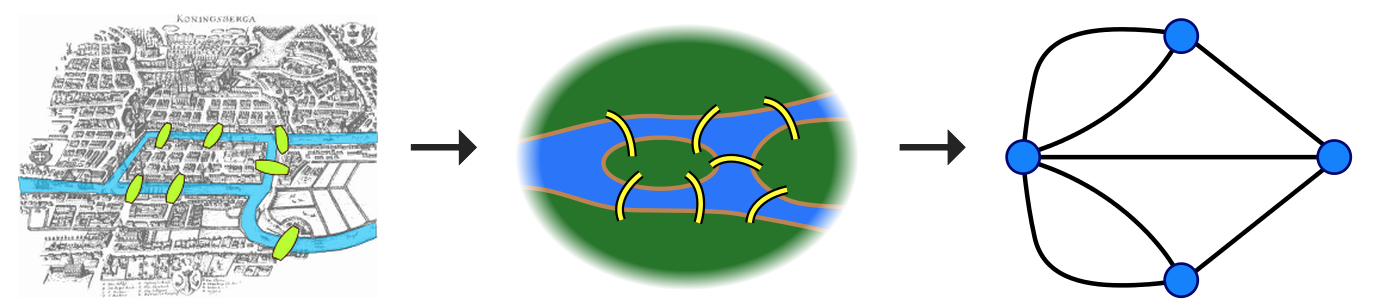
\includegraphics[width=\textwidth]{./img/konisberg.png}
\end{center}

Euler worked a bit on the problem, and saw that, in fact, he simply could invent graph theory to prove that there was no such path.

\subsection{Definitions}
\begin{itemize}
\item The degree of a node $v$, noted $\#v$, is the number of edges that are connected to this node. Edges that are loops (that connect a node to itself) count double.
\item An Eulerian path\footnote{Also called Eulerian trail} in a graph is a path that cross each edge of the graph once.
\item An Eulerian tour\footnote{Also called Eulerian cycle} is an Eulerian path that is also a cycle.
\end{itemize}

Euler then searched an Eulerian\footnote{yep, he was a bit self-centered} path in Königsberg.

\subsection{Properties}
After some hours thinking on the problem, he wrote some theorems:

\begin{itemize}
\item The sum of the degree for all nodes equals to two times the number of edges (all edges are linked to two nodes).
\item A graph contains an Eulerian tour if and only if all nodes have an even degree. \footnote{Here is the intuition for the demo: when you enter in a node, you "consume" one degree related to the inbound edge, and when you exit a node, you "consume" another degree related to the outbound edge. Thus, you consume two "part of degree" each time you go throughout a node.}
\item A graph contains an Eulerian path if and only if there is at most two nodes with an odd degree. 
\end{itemize}

\subsection{Hierholzer's Algorithm}
The Hierholzer's algorithm is used to find Eulerian tours\footnote{It can be easily expanded to find Eulerian paths: you just have to add an edge between the two nodes that have an odd degree, run the algorithm to produce the Eulerian tour, then delete the added edge!} in graph.

It is very simple: you simply start from a random vertex $u$, then follow one edge to another vertex (mark the edge as used), etc, until you reach again $u$. You have then formed a cycle that "uses" some of the edges. If there are still edges available on $u$, repeat the operation, and then merge the cycles, etc. If there are no longer unused edges starting from $u$, then go to the next vertex in the cycle, and repeat everything.

\begin{lstlisting}[label=code-eulerian,caption=Hierholzer's Algorithm, language=Java, tabsize=2, breaklines=true, numbers=left]
LinkedList<Integer> eulerianCycle(LinkedList<Integer>[] adj_list)
{
	//For simplicity, we assume that the graph is connected...
		
	LinkedList<Integer> cycle = new LinkedList<Integer>();
	cycle.add(0); //add an initial node
		
	//Iterate throught the cycle
	ListIterator<Integer> listIterator = cycle.listIterator();
    while (listIterator.hasNext())
    {
    	int new_start = listIterator.next();
    	//If we can begin a new cycle...
    	if(adj_list[new_start].size() != 0)
    	{
    		int current = new_start;
    		int size_added = 0;
    		do
    		{
    			int next_node = adj_list[current].poll();

				//delete the edge in the other direction
				//this is slow and can be improved using a separate Set
				adj_list[next_node].remove(new Integer(current));

				current = next_node;
				listIterator.add(current);
				size_added++;
			} while(current != new_start);

			//go back to the initial node, to verify there is no other edges
			for (int i = 0; i < size_added; i++)
				listIterator.previous();
		}
	}
	return cycle;
}
\end{lstlisting}

This algorithm runs in linear time, depending only of the number of vertices and edges: $O(|V|+|E|)$.

\subsection{Exercises}
\begin{enumerate}
\item Do the problem 10054 from UVA: \url{http://uva.onlinejudge.org/external/100/p10054.pdf}.
\textbf{Warning}: there is lot of input/output, so, in Java, use BufferedReader and BufferedWriter!
\item Bonus: do the problem 10596 from UVA: \url{http://uva.onlinejudge.org/index.php?option=com_onlinejudge&Itemid=8&category=24&page=show_problem&problem=1537}
\end{enumerate}